\chapter{Results and Discussion}

This chapter presents and analyses the results obtained from applying the \ac{ITM} on seismic waves. We first go through the travelling planar wave and then deal with
a velocity impulse point source. This chapter is split into three parts. As a starting point, the time-reversal is analysed in an acoustic media with an initial condition
as a travelling planar P-Wave. The second part deals with the time-reversal of a velocity impulse point source in an Acoustic media. The third part deals with the time-Reversal
of a velocity impulse point source in an Elastic Media with refocusing of both P- and S- waves together and separately. In all the cases, we check if the refocused
wave will converge to the location of the source as we expect the reversed wave to have the same speed as the original wave. \\

We analyse all cases with a homogenous medium to deliver on a sound proof of concept of the \ac{ITM} being useful to refocus different kind of waves. We used a modification
of our benchmark test problem, WP2-LOH1 to show refocusing in realistic media.

\section{Time-reversal of a travelling planar P-wave}
The acoustic case is a simplification of propagation in an elastic media. The second Lam\'{e} parameter $\mu$ is set to zero. The medium is characterized by the following parameters

\begin{equation}
    \rho = 4, \mu = 0, \lambda = 1 ,
\end{equation}

The propagation speed of the P-wave in this case is given by

\begin{equation}
    v_p = \sqrt{\frac{\lambda + 2 \mu}{\rho}} = \sqrt{\frac{1}{4}} = \frac{1}{2} .
\end{equation}

We impose an initial condition such that there is a P-Wave travelling towards the negative X-axis. The details on how the initial conditions are set up to ensure a left going P- wave is discussed in
\href{https://seissol.readthedocs.io/en/latest/initial-condition.html#travelling-wave}{Travelling Wave: SeisSol}. We impose a P-Wave with a wavelength of 
$\lambda = 1.0$. This gives us a timeperiod of $T=2.0$. We choose a cubic computational domain of [-1, 1] in all three directions with periodic boundary conditions with the mesh shown in figure \ref{fig:acoustic_mesh} with
163840 triangular elements. 

\begin{figure}
    \centering
    \includegraphics[width=\linewidth]{figures/mesh_cube.png}
    \caption{Mesh used for the acoustic case}
    \label{fig:acoustic_mesh}
\end{figure}

We start our initial travelling wave at the origin and our wave travels to the boundary in $t = \frac{1}{2}$. We start our \ac{ITM} at $t=2$ such that the reversed wave will travel back to the origin at $t=4.0$ to meet the
forward going wave. 

\begin{figure}
    \centering
    \begin{subfigure}[b]{0.475\textwidth}
        \centering
        \includegraphics[width=\textwidth]{figures/travellingwave_t0.png}
        \caption{t=0} 
    \end{subfigure}
    \vskip\baselineskip
    \begin{subfigure}[b]{0.475\textwidth}   
        \centering 
        \includegraphics[width=\textwidth]{figures/travellingwave_t1.png}
        \caption{t=1.0}
    \end{subfigure}
    \hfill
    \begin{subfigure}[b]{0.475\textwidth}   
        \centering 
        \includegraphics[width=\textwidth]{figures/travellingwave_t2.png}
        \caption{t=2.0}
    \end{subfigure}
    \vskip\baselineskip
    \begin{subfigure}[b]{0.475\textwidth}   
        \centering 
        \includegraphics[width=\textwidth]{figures/travellingwave_t3.png}
        \caption{{t=3.0}}
    \end{subfigure}
    \hfill
    \begin{subfigure}[b]{0.475\textwidth}   
        \centering 
        \includegraphics[width=\textwidth]{figures/travellingwave_t4.png}
        \caption{{t=4.0}}
    \end{subfigure}
    \caption{\ac{ITM} applied on a travelling planar P-wave in an acoustic media.}
\end{figure}

Here, we notice that there is a reflection of the forward going wave and it meets the the forward going wave at the origin at $t=4.0$. This is a proof of concept that the \ac{ITM} can be used to refocus waves in an acoustic media. \\

To observe the refocusing in a clearer way, we choose a slice perpendicular to the Z-axis at $x=0$ and plot the wavefield in terms of u-velocity along the x-axis
at different times.We can see that at $t=2.0$, there is a reflected component along with the forward component. At $t=3.0$ i.e., half the time-period after
the application of the \ac{ITM}, we notice that the reflected component interacts with the forward wave for the first time. This shows that in half the time-period, the reflected wave travelled half the wave length interacting
with the forward travelling wave. At $t=4.0$, we notice that the reflected wave has travelled the entire wave length and is refocused at the origin. 
This is shown in figure \ref{fig:space-timeplot-travelling}.

\begin{figure}
    \centering
    \includegraphics[width=0.75\linewidth]{figures/space-time-plot-travelling.pdf}
    \caption{Space Time plot for Acoustic Travelling Wave with \ac{ITM}}
    \label{fig:space-timeplot-travelling}
\end{figure}

\section{Time-reversal of a velocity impulse point source in an Acoustic media} \label{sec:acousticITM}

We now consider a velocity impulse point source in an acoustic media. We pick the Lam\'{e} parameter $\lambda$, density $\rho$ 
from the half-space of the benchmark case WP2-LOH1~\footnote[1]{https://seissol.readthedocs.io/en/latest/pointsource.html} to make it a homogenous acoustic medium. 
The medium is characterized by the following parameters

\begin{align}
    \begin{split}
        \rho &=    2700.0 \\
        \mu &=     0.0 \\
        \lambda &= 3.24038016e10 ,
    \end{split}
\end{align}

This makes the velocity of the P-wave to be

\begin{equation}
    v_p = \sqrt{\frac{3.24038016e10}{2700}} \approx 3464 .
\end{equation}

We choose a computational domain of [-26000,32000] X [-26000,32000] X [0,34000] and a simulation time of $t=10.0$ with \ac{ITM} applied at $t=5.0$ 
such that the originating waves do not reflect back from the boundaries at the X- and Y- axis ensuring that
reflections due to \ac{ITM} are clearly noticeable when we take a slice perpendicular to Z- axis. 
Our velocity impulse source is at [3000,3000,17000] such that it is exactly at the center of the domain. 
We choose an unstructured mesh with tetrahedral elements with 1391713 elements such that there are more elements near the source to capture the steep gradients like shown in 
figure \ref{fig:mesh-loh1}.

\begin{figure}
    \centering
    \includegraphics[width=\linewidth]{figures/mesh_loh1.png}
    \caption{Sample Mesh for Velocity Impulse Point Source Simulations}
    \label{fig:mesh-loh1}
\end{figure}

We apply a source such that it dies exponentially with time multiplied with a constant. It is then applied in equation \ref{eq:setofequations} as per the direction
it is applied to. We use the following formulation for the source term

\begin{align}
    \begin{split}
        \dot{S} = \frac{1}{T^2} t e^{-\frac{t}{T}} \\
        S_i = \dot{S} \times C_i ,
    \end{split}
    \label{eq:source}
\end{align}

where T is a constant to decide the duration of the source approximately. We choose T=0.1. $i$ is the direction of the source. 
We choose the source to be in the Z-direction which makes $C_x = 0, C_y = 0, C_z = 1.2e16$. With this, our source looks like in figure \ref{fig:source}

\begin{figure}
    \centering
    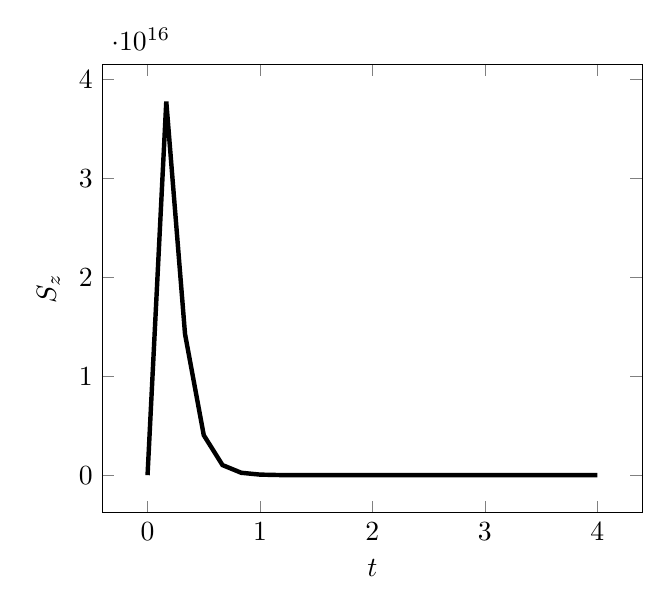
\begin{tikzpicture}[scale=1.0]
        \begin{axis}[
            ylabel = $S_z$,
            xlabel = $t$]
            \addplot[domain=0:4, black, ultra thick]{1.2e16 * x*exp(-x/0.1)/(0.1*0.1)};
        \end{axis}
    \end{tikzpicture}
    \caption{Source term used for Velocity Impulse Point Source}
    \label{fig:source}
\end{figure}

We pick a slice at $Z=20000$ i.e., 3000 away from the source location in Z-direction.
We visualise the wavefield with velocity in X-direction. With this setup and velocity impulse, we see that the velocity in X-direction
looks like in figure \ref{fig:space-timeplot-acousticnoITM}

\begin{figure}
    \centering
    \includegraphics[width=0.75\linewidth]{figures/Acoustic-noITM.pdf}
    \caption{Space Time plot for Wave produced by Velocity Impulse Point Source in Acoustic Media}
    \label{fig:space-timeplot-acousticnoITM}
\end{figure}

We notice that we have only one wave propagating in time as expected as we have an acoustic media and it reaches our slice around 1.5 seconds. We notice another 
strange static velocity near the source which is not expected and yet to be made sense of with the package. But it does not affect our refocusing and has nothing to do with
our application of \ac{ITM}. We now apply ITM on the same setup at $t=5.0$. We notice that the wavefield looks like in figure \ref{fig:space-timeplot-acousticITM}

\begin{figure}
\begin{subfigure}[b]{0.49\textwidth}   
    \centering 
    \includegraphics[width=\textwidth]{figures/AcousticITM.pdf}
    \caption{Wave produced by Velocity Impulse in Acoustic Media with \ac{ITM}}
\end{subfigure}
\hfill
\begin{subfigure}[b]{0.49\textwidth}   
    \centering 
    \includegraphics[width=\textwidth]{figures/AcousticITMAnnotated.pdf}
    \caption{Expected location of forward and reflected waves in Time}
    \label{subfig:acousticITMAnnotated}
\end{subfigure}
\caption{Space Time plot for Wave produced by Velocity Impulse Point Source in Acoustic Media with \ac{ITM}}
\label{fig:space-timeplot-acousticITM}
\end{figure}

We notice that there is a reflected wave travelling back to the source. We notice that the reflected wave leaves our slice around $t=8.5$ showing that the reflected wave
is reflected along the line $t=5.0$ which is our point in time when we applied the \ac{ITM}. In figure \ref{fig:space-timeplot-acousticITM}, we plot the expected
location of the wave front from the forward going and reflected waves assuming spherical waves being generated at the source and that the reflected wave is spherical
and has the same speed as the original incident wave in figure \ref{subfig:acousticITMAnnotated}. This confirms that the application of \ac{ITM} produces a reflected wave
successfully in Acoustic Media. \\

\section{Time-reversal of a velocity impulse point source in an Elastic media} \label{sec:elasticITM}
We now consider a velocity impulse point source like in Section \ref{sec:acousticITM}. We choose the material parameters from the half-space of the 
benchmark case WP2-LOH1~\footnote[1]{https://seissol.readthedocs.io/en/latest/pointsource.html} to make it a homogenous elastic medium. The material parameters 
are characterized by

\begin{align}
    \begin{split}
        \rho &=    2700.0 \\
        \mu &=     3.23980992e10 \\
        \lambda &= 3.24038016e10 ,
    \end{split}
\end{align}

which makes the velocities of P- and S- waves to be

\begin{align}
    \begin{split}
        v_p &= 6000.0 \\
        v_s &= 3464.0 .
    \end{split}
\end{align}

In this case we extend our computational domain even further to [-104000,128000] X [-104000,128000] X [0,136000] and a simulation time of $t=18.0$ with \ac{ITM} applied at $t=9.0$
such that the originating waves do not reflect back from the boundaries at the X- and Y- axis ensuring that reflections due to the \ac{ITM} are clearly noticeable when we take a slice perpendicular to Z- axis.
Our velocity impulse source is at [12000,12000,68000] such that it is exactly at the center of the domain.
We chose to analyse the simulation for a longer time in this scenario as the velocities of P- and S- waves are different and the P- wave travels farther quickly when compared to 
the S- wave. We choose an unstructured mesh with tetrahedral elements with 12646379 elements similar to the Acoustic Case such that there are more elements near the source
to capture the steep gradients near the Source. We apply a source which has already been discussed in equation \ref{eq:source} and figure \ref{fig:source}. \\

We pick a slice at $Z = 40000$ and visualise the wavefield with velocity in X-direction and the displacement along the X-axis. With this setup and velocity impulse, 
we see that the velocity in X-direction looks like in figure \ref{fig:space-timeplot-elasticnoITM}.

\begin{figure}
    \centering
    \includegraphics[width=0.75\linewidth]{figures/noITMElasticvelocity.pdf}
    \caption{Space Time plot for Waves produced by Velocity Impulse Point Source in Elastic Media}
    \label{fig:space-timeplot-elasticnoITM}
\end{figure}

We integrate the obtained velocity field to plot displacement field in X- direction as shown in figure \ref{fig:space-timeplot-elasticnoITMdisplacement}.

\begin{figure}
    \centering
    \includegraphics[width=0.75\linewidth]{figures/noITMElasticdisplacement.pdf}
    \caption{Space Time plot for Waves produced by Velocity Impulse Point Source in Elastic Media in displacement}
    \label{fig:space-timeplot-elasticnoITMdisplacement}
\end{figure}

We can clearly notice two propagating waves as expected as we are dealing with an elastic media now. We notice a static displacement field in between the two waves.
This is a common phenomenon in displacement fields built with simulation codes in seismic simulations(cite?). 
We now apply \ac{ITM} on the same setup at $t=9.0$. We notice that the wavefield looks like in figure \ref{fig:space-timeplot-elasticITM}

\begin{figure}
    \centering
    \includegraphics[width=0.75\linewidth]{figures/Elastic-tworeflections.pdf}
    \caption{Space Time plot for Waves produced by Velocity Impulse Point Source in Elastic Media with \ac{ITM}}
    \label{fig:space-timeplot-elasticITM}
\end{figure}

We notice that there are two clearly reflected waves travelling back to the source. We notice that the faster moving wave i.e., P-wave leaves our slice around 
$t=13.0$ which is around 4 seconds after the application of \ac{ITM} which is the time it travelled through the slice just before the application of \ac{ITM}. 
We notice that the slower moving wave i.e., S-wave also has a reflection symmetric about line $t=9.0$. We now plot the displacement plot in x-direction on the 
slice just like we did in figure \ref{fig:space-timeplot-elasticnoITMdisplacement} in \ref{fig:space-timeplot-elasticITMdisplacement}.

\begin{figure}
    \centering
    \includegraphics[width=0.75\linewidth]{figures/Elastic-tworeflections-displacement.pdf}
    \caption{Space Time plot for Waves produced by Velocity Impulse Point Source in Elastic Media with \ac{ITM} in displacement}
    \label{fig:space-timeplot-elasticITMdisplacement}
\end{figure}

We can clearly see two reflections even in case of displacement wave field too and the static displacements between the two waves persist. But we see extra features
here in case of displacement wave-field. We obtain extra static displacements in time as vertical streaks which originate from the point where the waves meet the slice
at \ac{ITM}. These are not yet explained but we suspect they may be explained either by the physical phemonenon or due to the numerical implementation or due to errors
produced to numerical integration of the velocity wavefields. \\

This shows that both the waves can be reflected simultaneously by scaling the material parameters to change their impedance to obtain a component which 
is reflected back to its source. \\

\section{Time-reversal of P- wave of a velocity impulse point source in an Elastic media} \label{sec:elasticITMpwave}
We now demonstrate the reflection of just the P- wave by scaling the Lam\'{e} parameter $\lambda$ and keeping the second Lam\'{e} parameter $\mu$ constant.\\
The same setup is used as in Section \ref{sec:elasticITM} and we try to reflect just the P- wave while letting the S- wave travel unaffected in time. The slice
and everything else about the simulation remain the same. The wavefields without \ac{ITM} looks like in figures \ref{fig:space-timeplot-elasticnoITM} and
\ref{fig:space-timeplot-elasticnoITMdisplacement}

\begin{figure}
    \centering
    \includegraphics[width=0.75\linewidth]{figures/pwave-ITM1.pdf}
    \caption{Reflection of P- wave in Elastic Media with \ac{ITM}}
    \label{fig:space-timeplot-pwave}
\end{figure}

After the application of the \ac{ITM}, we see reflections in the wavefield in figure \ref{fig:space-timeplot-pwave}.
As the reflection in figure \ref{fig:space-timeplot-pwave} is seen but is faint. We plot the same with a different colorbar just to show the reflection in a clearer
way in figure \ref{fig:space-timeplot-pwave2}

\begin{figure} %% replace pictures. Not clear and being cut
    \centering
    \includegraphics[width=0.75\linewidth]{figures/pwave-ITM2.pdf}
    \caption{Reflection of P- wave in Elastic Media with \ac{ITM}}
    \label{fig:space-timeplot-pwave2}
\end{figure}

We can clearly see here in this plot that there is a P- wave which is reflected without affecting the S- wave. This provides us a proof of concept where we 
can reflect one wave by changing its impedance while maintaining the other wave's impedance constant. \\

\begin{figure} %% replace pictures. Not clear and being cut
    \centering
    \includegraphics[width=0.75\linewidth]{figures/pwave-ITMdisplacement.pdf}
    \caption{Reflection of P- wave in Elastic Media with \ac{ITM} in displacement}
    \label{fig:space-timeplot-pwavedisplacement}
\end{figure}

We plot the displacement wavefield in figure \ref{fig:space-timeplot-pwavedisplacement} and we can see the reflected P- wave in displacement wavefield and the static
displacement is noticed in this case too just like in the case of reflecting both the waves. 

\section{Time-reversal of S-wave of a velocity impulse point source in an Elastic media}
Just like in Section \ref{sec:elasticITMpwave}, we now demonstrate the reflection of just the S- wave by modifying the Lam\'{e} parameters such that P-wave does not
get reflected but the S- wave does. The same setup is used as in section \ref{sec:elasticITM} and we try to reflect just the S- wave while letting the P- wave travel
unaffected in time. The slice and everything else about the simualtion remain the same. The wavefields without \ac{ITM} looks like in figures in \ref{fig:space-timeplot-elasticnoITM}
and \ref{fig:space-timeplot-elasticnoITMdisplacement}. \\

After the application of the \ac{ITM}, we see reflections in the wavefield in figure \ref{fig:space-timeplot-swave} showing the zoomed version near the 
\ac{ITM} so that the reflected part is clearly visible in subfigure \ref{subfig:swavezoomed}.

\begin{figure}
    \begin{subfigure}[b]{0.49\textwidth}   
        \centering 
        \includegraphics[width=\textwidth]{figures/swaveITM1.pdf}
        \caption{Reflecting S-waves in Elastic media}
        \label{subfig:swave}
    \end{subfigure}
    \hfill
    \begin{subfigure}[b]{0.49\textwidth}   
        \centering 
        \includegraphics[width=\textwidth]{figures/swaveITM2.pdf}
        \caption{Zoomed cut section}
        \label{subfig:swavezoomed}
    \end{subfigure}
    \caption{Reflection of S- wave in Elastic Media with \ac{ITM}}
    \label{fig:space-timeplot-swave}
\end{figure}
    
We plot the displacement wavefield in figure \ref{fig:space-timeplot-swavedisplacement} and we can see the reflected S- wave in displacement 
wavefield and the static displacement like in previous section persists. We need more investigation into this to make sense of this static displacement.

\begin{figure}
    \centering
    \includegraphics[width=0.75\linewidth]{figures/swaveITMdisplacement.pdf}
    \caption{Reflection of S- wave in Elastic Media with \ac{ITM} in displacement}
    \label{fig:space-timeplot-swavedisplacement}
\end{figure}

We can clearly see here in this plot that there is a S- wave which is reflected without affecting the P- wave. 
This provides us a proof of concept where we show that we can reflect one wave by changing its impedance while maintaining the other wave's impedance constant. \\

\section{Convergence Test}
We now perform a convergence test to check for the correctness of our implementation of the \ac{ITM} is convergent with our \ac{ADER}-\ac{DG} scheme. 
We check the error between our numerical implementation and the analytical solution developed in Section \ref{section:ITMAcoustic}. We use
